\section{Vererbung}
Die Vererbung funktioniert in Java ähnlich wie in C++. Eine Klasse in Java kann jedoch nur \textbf{eine} Basisklasse haben.
Eine abgeleitete Klasse erbt die Instanzvariablen und Instanzmethoden der Basisklasse.
Die oberste Klasse aller Basisklassen ist \verb|Object|. Methoden von \verb|Object| sind:
\begin{itemize}
    \itemsep0em
    \item \verb|public String toString()|
    \item \verb|public boolean equals(Object obj)|
    \item \verb|public int hashCode()|
    \item ...
\end{itemize}

\subsection{Impliziter Code in Vererbung}
\begin{center}
    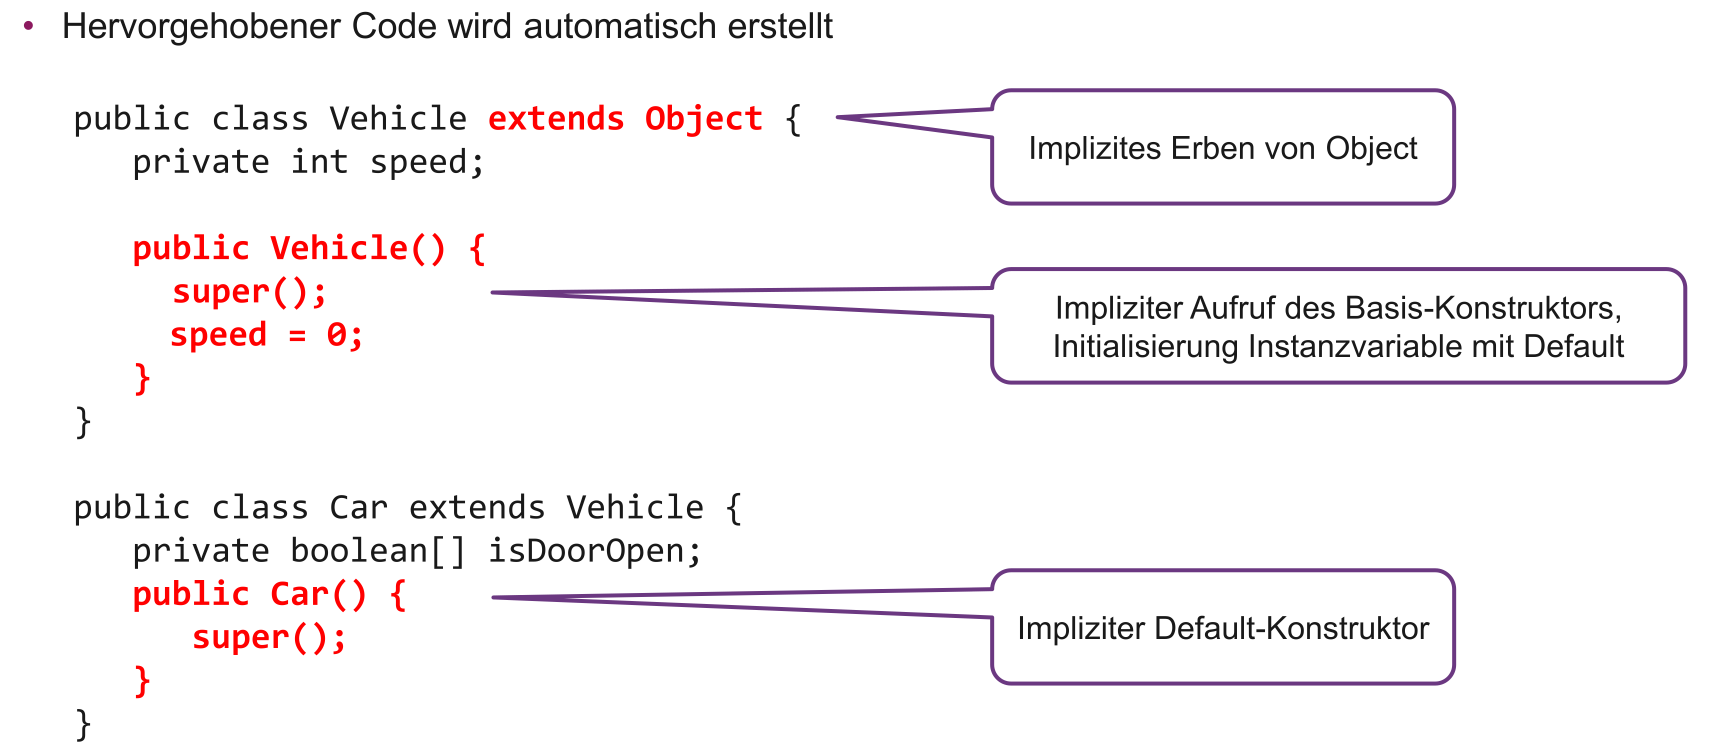
\includegraphics[width=0.9\columnwidth]{pictures/vererbung-implizit.png}
\end{center}

\subsection{Konstruktor bei Vererbung}
\begin{center}
    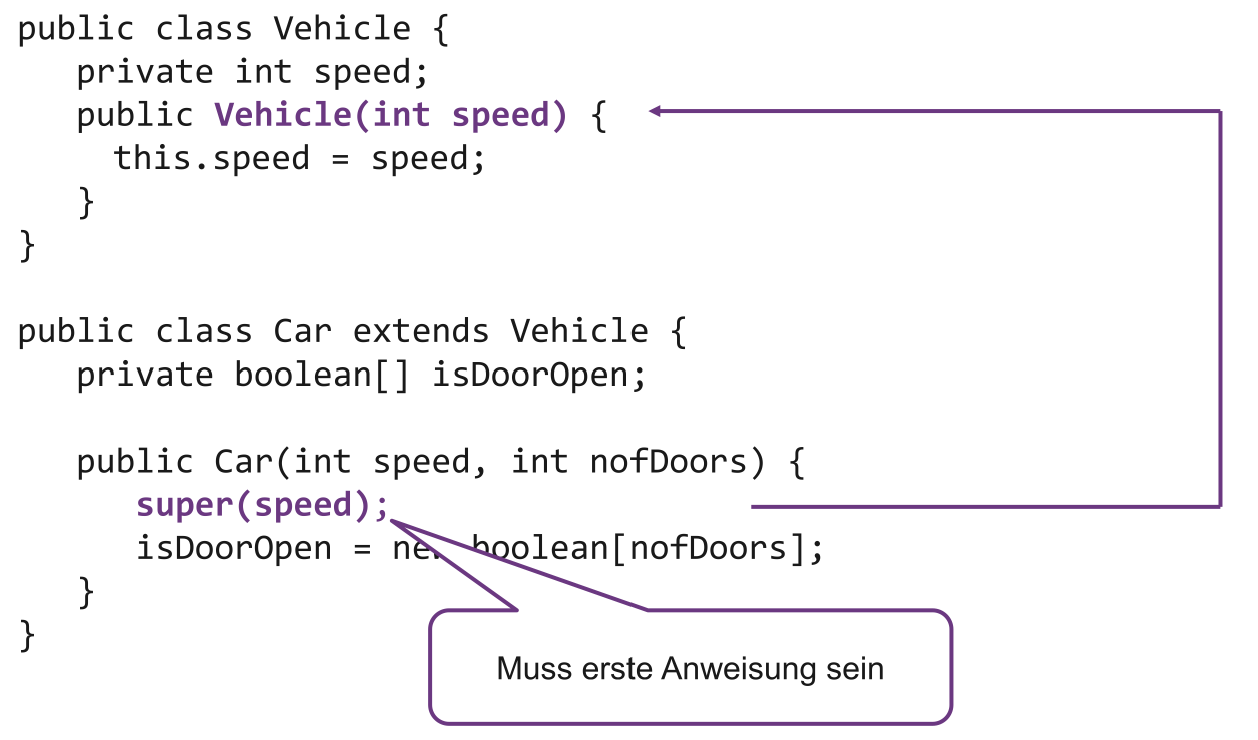
\includegraphics[width=0.9\columnwidth]{pictures/vererbung-konstr.png}
\end{center}

\subsection{Overriden von Methoden}
Gleiche Funktion wie das Keyword \verb|virtual| in C++, dieses gibt es jedoch nicht in Java. Stattdessen wird
vor einer neu implementierten Methode einer Subklasse das Schlüsselwort \verb|@Override| gesetzt. Dies ist optional, aber sinnvoll.\\
\verb|@Override|\\
\verb|public void print()|\\

Mit \verb|super| wir eine überschriebene Methode aufgerufen.
\begin{center}
    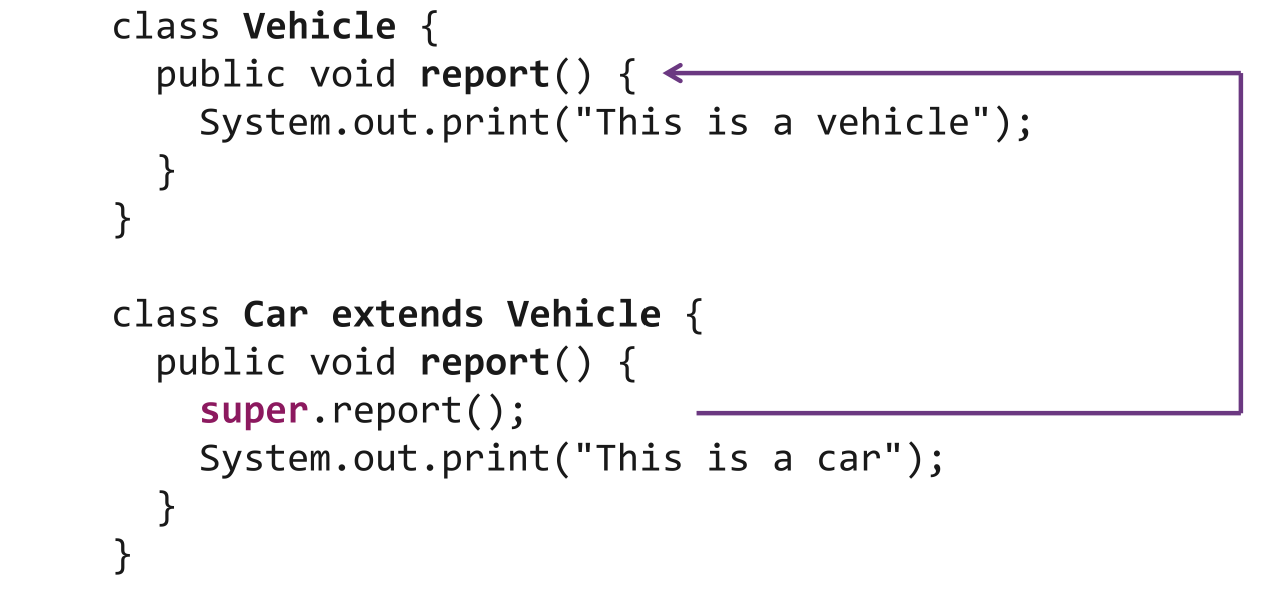
\includegraphics[width=0.9\columnwidth]{pictures/super.png}
\end{center}

\subsection{Abstrakte Klassen}{\label{AbstractClass}}
Schlüsselwort: \verb|abstract|\\

Eine abstrakte Klasse ist nicht vollständig implementiert, sprich einzelne Methoden können nicht implementiert 
sein und die Klasse kann nicht instanziiert werden.

Sie dient als Basistyp für Sub-Klassen (statischer Typ) und vererbt ihre Grundfunktionalität an Sub-Klassen.\\
Beispiel:\\
\begin{minipage}{0.5\columnwidth}
    \begin{center}
        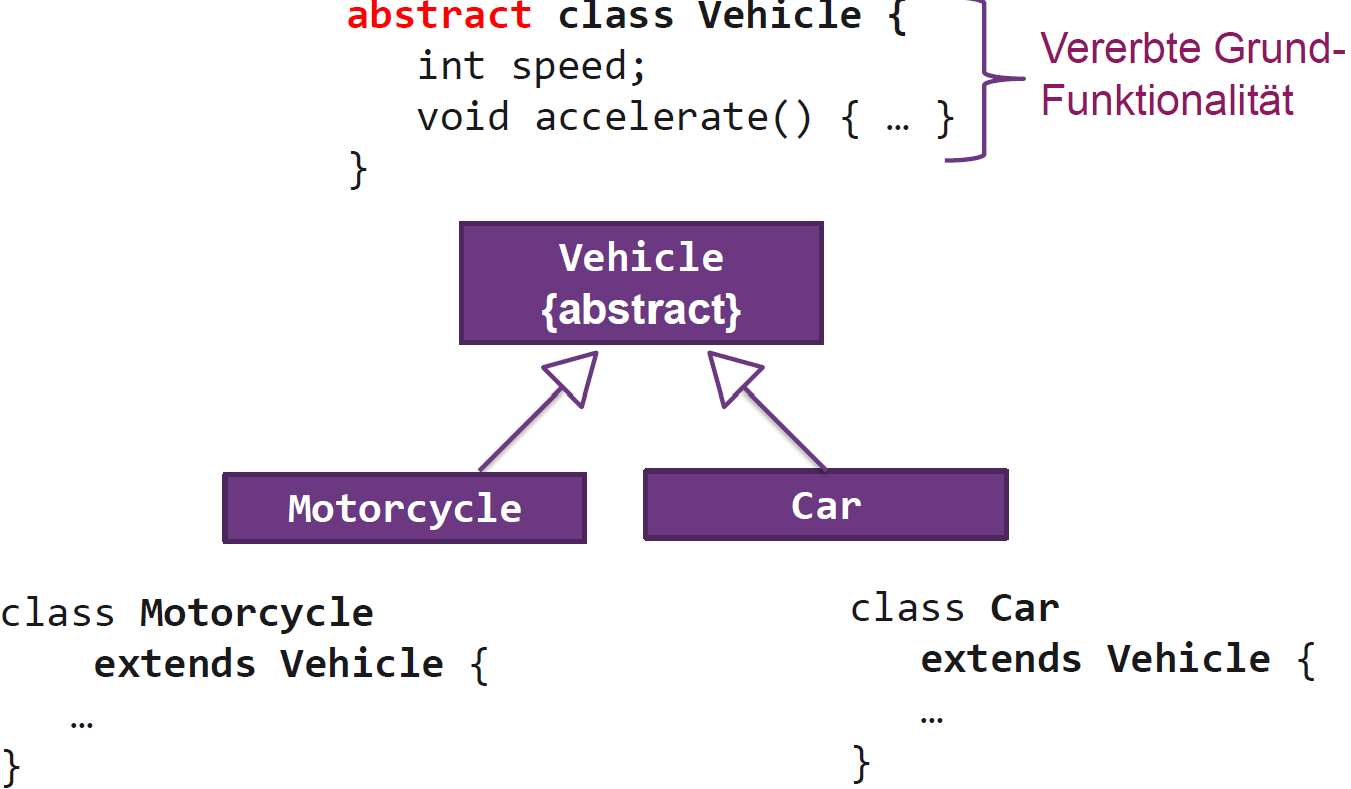
\includegraphics[width=0.9\columnwidth]{pictures/abstrakte-Klasse-Bsp.png}
    \end{center}
\end{minipage}
\hfill
\begin{minipage}{0.5\columnwidth}
    \begin{center}
        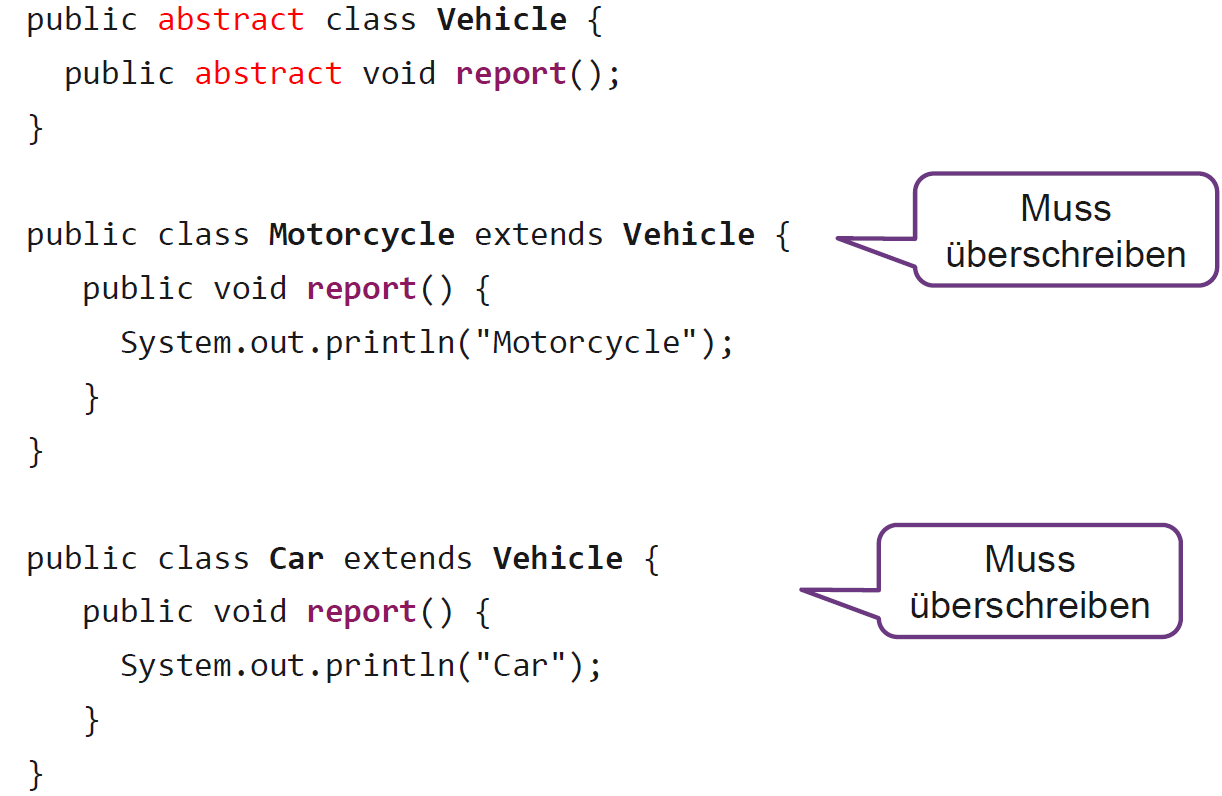
\includegraphics[width=0.9\columnwidth]{pictures/abstrakte-Klasse-Bsp2.png}
    \end{center}
\end{minipage}

\section{Binding}
\subsection{Dynamic Binding}
Generell bei nicht-privaten Instanzmethoden

\subsection{Static Binding}
Generell bei privaten Instanzmethoden (In Subklasse nicht mehr sichtbar $\rightarrow$ Neudef. der Methode) und statischen Methoden


